\newsection
\subsection{Reasoning and search}
\label{sec:reasoning}
\sectionauthors{Yuhuai Wu, Frieda Rong, Hongyu Ren, Sang Michael Xie, Xuechen Li, Andy Shih, Drew A. Hudson, Omar Khattab}


\begin{figure}[!ht]
\centering
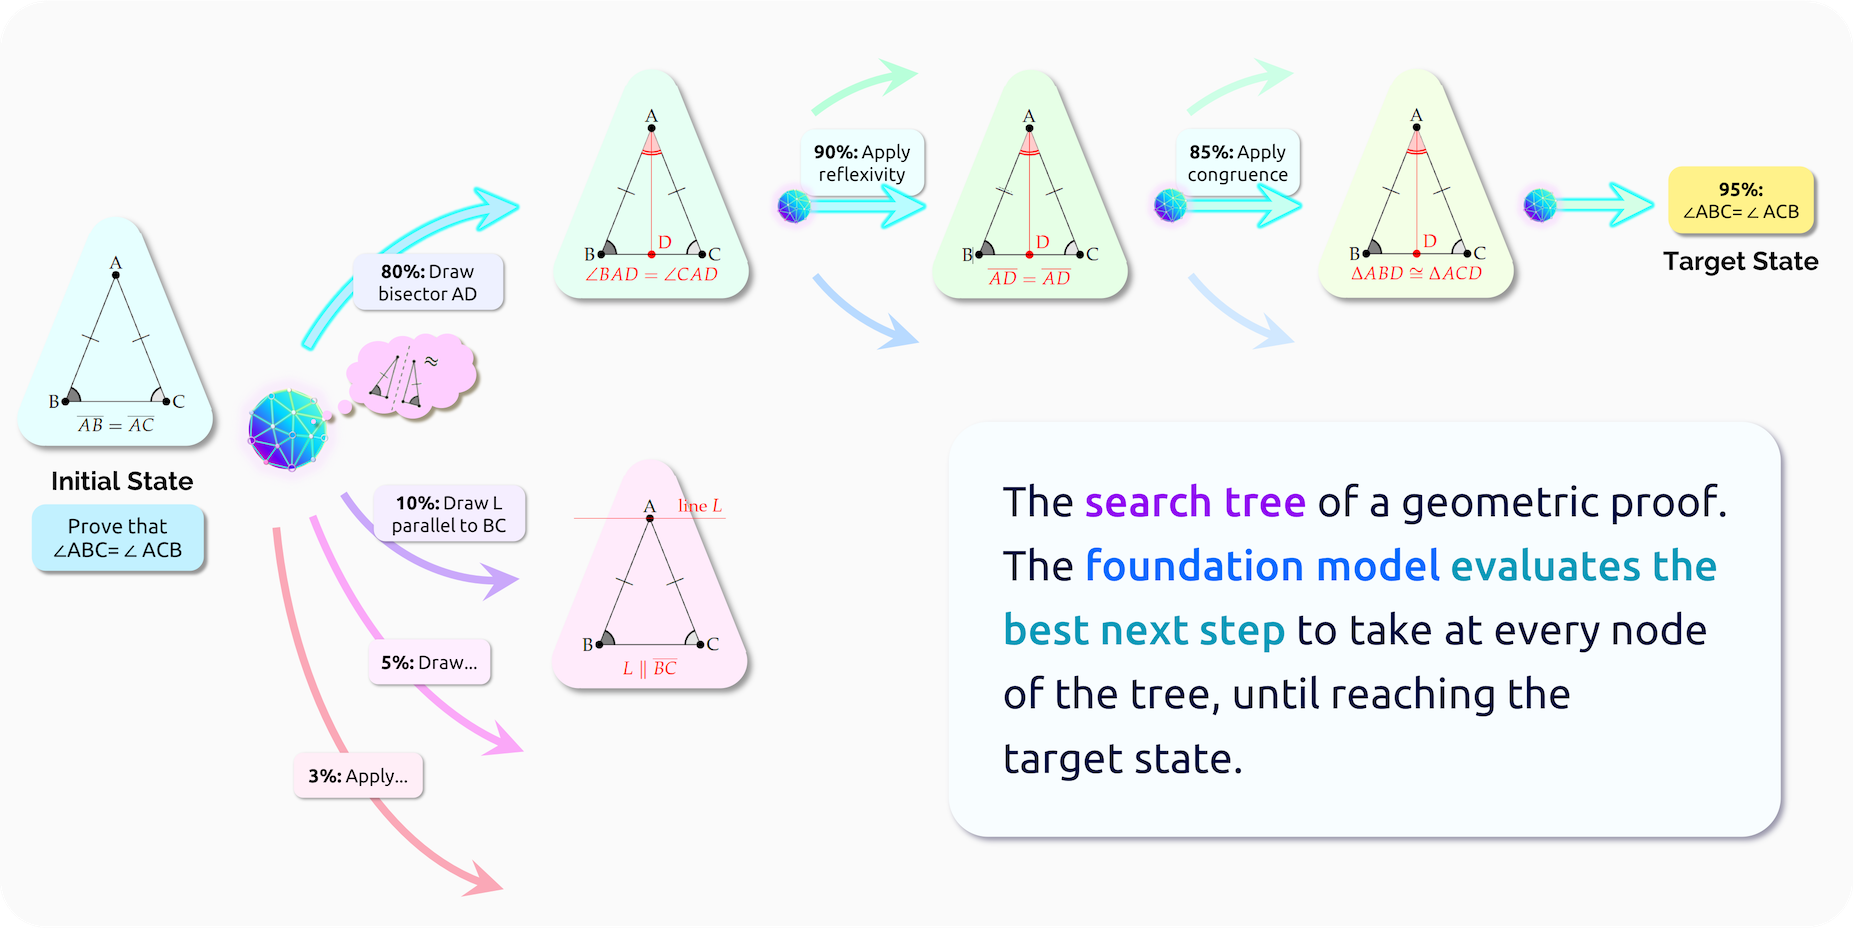
\includegraphics[width=\linewidth]{capabilities/figures/Reasoning_1.png}
\caption{\label{fig:reasoning-geometry} Multimodality can allow foundation models to not only reason with formal symbolic language, but also exploit \emph{visual aspects} of the problem, such as equivalence, symmetry, and Euclidean geometry, to prune the infinite search space and find promising constructions for a solution (\refsec{reasoning-tasks}), mimicking the way humans reason about geometry problems.}
\end{figure}

Reasoning and search have been a central theme throughout the history of AI. Classic tests of intellect, from strategy games to abstract mathematical discovery, served as inspirational goal posts that pushed the limits of ``machine intelligence'' through a need to devise ever smarter ways of searching for winning solutions.
In the early days, symbolic methods were the dominant approach for reasoning~\citep{DBLP:books/aw/RN2020}, but the involved engineering effort and the need to formalize heuristics to tackle intractable search spaces quickly proved cumbersome. 
More recently, data-driven methods using neural networks have shown encouraging results\dash{}\eg defeating the best humans in Go~\citep{DBLP:journals/nature/SilverHMGSDSAPL16}, a board game with a much larger space of actions than the classic challenge of chess\dash{}by exploiting statistical structures and learning useful heuristics.
This section outlines existing reasoning tasks, ones that require scaling to ever-larger search spaces and understanding the world broadly (\refsec{reasoning-tasks}).
We then argue in \refsec{reasoning-role} that foundation models should play a central role towards general reasoning as vehicles for capturing the statistical regularities of unbounded search spaces (\emph{generativity}), allowing positive transfer across tasks and scenarios (\emph{universality}), and exploiting the grounding of knowledge in multi-modal environments (\emph{grounding}). 

\subsubsection{What are the current tasks?}
\label{sec:reasoning-tasks}

Many reasoning problems pose unbounded search spaces, where systems must deal with numerous kinds of open-ended alternatives. Consider trying to prove that the angles $\angle B$ and $\angle C$ are equal for an isosceles triangle $\triangle ABC$ with $AB=AC$ (\reffig{reasoning-geometry}). A system can perform any number of actions \textit{at each step of reasoning}. For instance, the system could add a new auxiliary point with an arbitrary construction, say a perpendicular line, a parallel line, or a tangent circle, and the search space only grows larger as the diagram grows more complicated. One way to prove this theorem is to draw a line $AD$ that is the angle bisector of $A$, and use the congruence of the two triangles $\triangle ABD$ and $\triangle ACD$ to show $\angle B = \angle C$, but how can systems find this without extensive search?

More generally, a mathematician is not confined with searching in diagram constructions and Euclidean theorems: mathematicians can apply a vast number of theorems from various branches of mathematics, make high-level conjectures, formalize new mathematical concepts, or find counterexamples. This contrasts with more structured AI challenges such as the game of Go, whose search space is considered much smaller.\footnote{Less than the number of grid points on the Go board (\ie 361 actions for a 19$\times$19 board).}

Besides theorem proving, many real-world problems deal with unbounded search spaces, such as program synthesis~\citep{DBLP:journals/ftpl/GulwaniPS17}, drug discovery~\citep{Drews2000DrugDA}, chemical synthesis~\citep{DBLP:journals/nature/SeglerPW18}, computer-aided design~\citep{computer_aided_design}, combinatorial optimization~\citep{DBLP:journals/eor/BengioLP21}, and more. 
These reasoning problems tend to exhibit similar structure, like the bijection between retrosynthesis in drug discovery and theorem proving in propositional logic, illustrated in \reffig{reasoning-retrosynthesis}: in both problems, one is building a tree of synthesis, whose nodes are chemical products on the one side and propositions on the other, and the leaf nodes are the products on the one side, and end axioms on the other. 
In these problems, a simulated environment is often provided, which allows a solver to run several search threads towards building the solution tree. The simulator often provides intermediate feedback, say, informing the solver with the remaining propositions to establish before the proof is considered complete. The solver in turn needs to select the most promising search thread and proceed based on the intermediate feedback.

\begin{figure}[t]
\centering
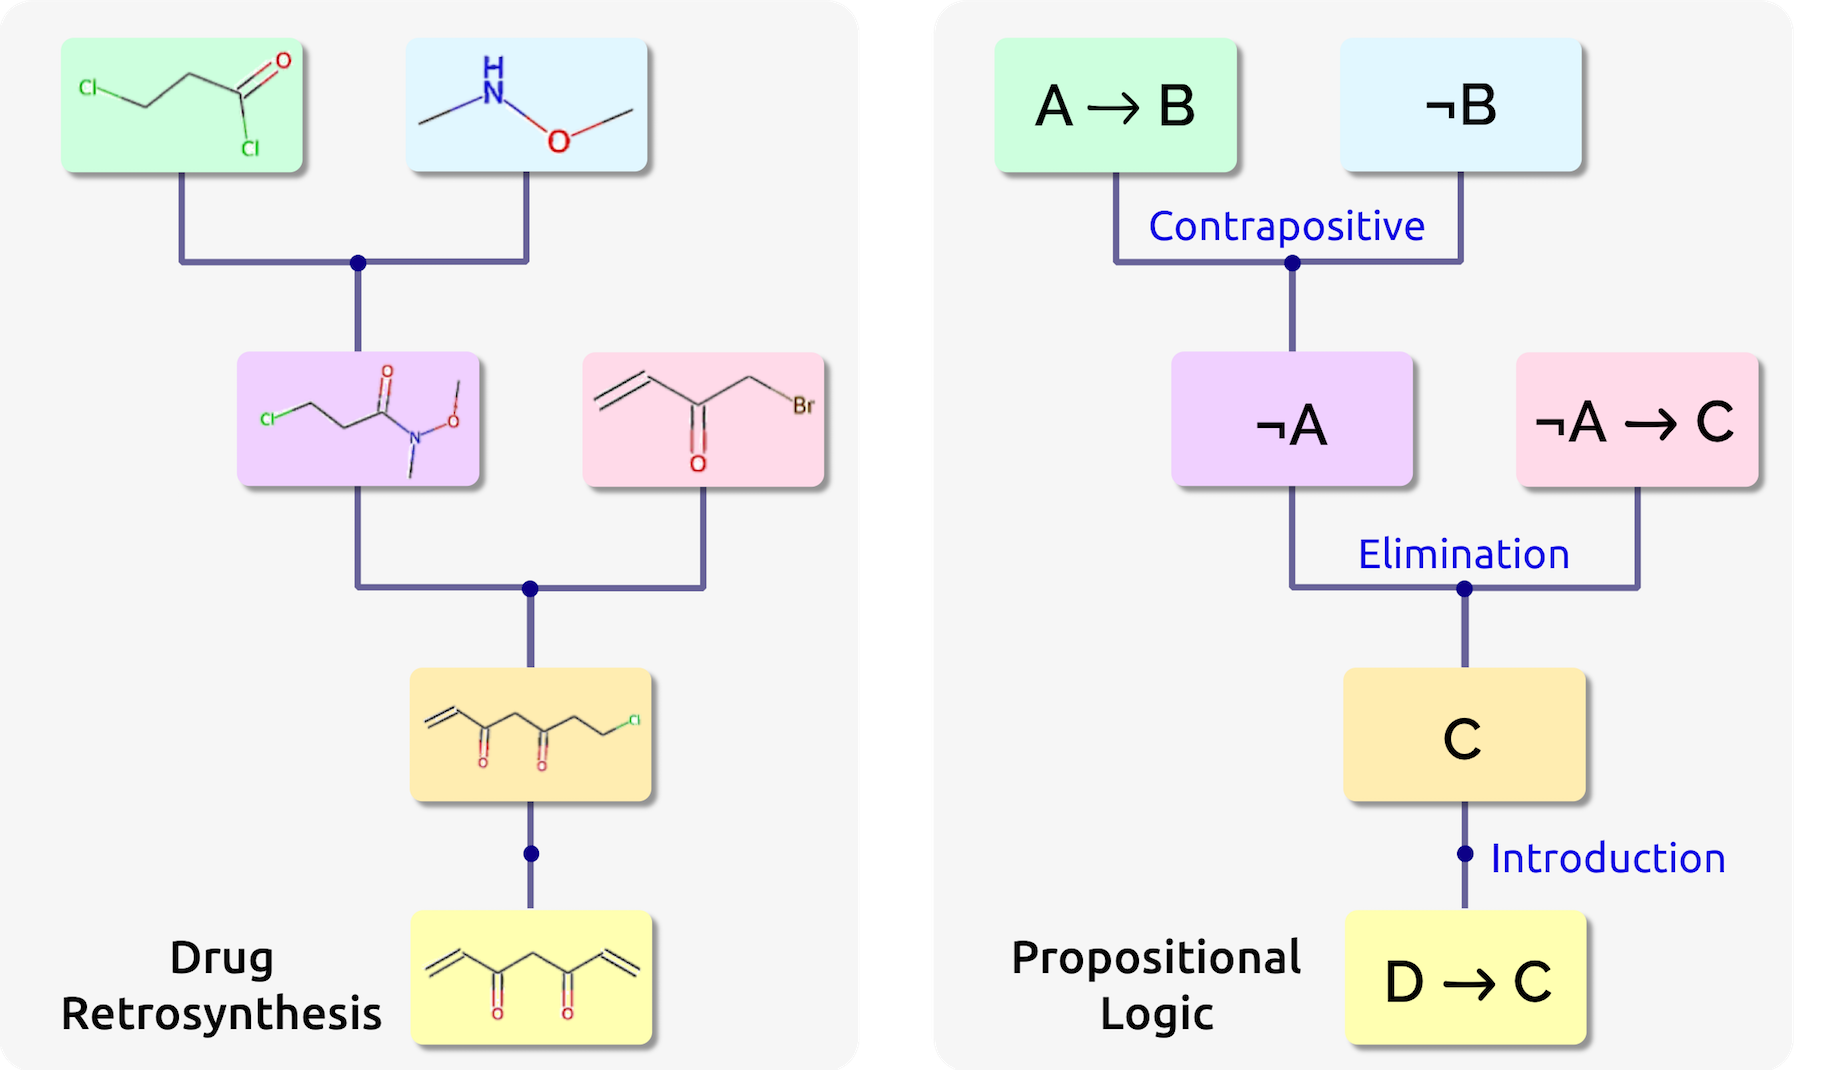
\includegraphics[scale=0.35]{capabilities/figures/Reasoning_2.png}
\caption{\label{fig:reasoning-retrosynthesis} \textbf{Left:} A reaction route for 1,6-Heptadiene-3,5-dione predicted by machine learning-based drug retrosynthesis planner AiZynthFinder \cite{genheden2020retrosynthesis,yoshikawa2021retrosynthesis-twitter}. \textbf{Right:} A sample proof tree in propositional logic where the formulas outlined in green represent axioms. Although they arise from different domains, both trees are structurally the same.}
\end{figure}

Recently, there has been a surge of interest in applying learning-based approaches to tackle reasoning problems. 
To overcome the unbounded search space challenge, researchers first started with a constrained search space to make the problem tractable~\citep{DBLP:journals/corr/abs-1806-00608, DBLP:conf/icml/BansalLRSW19}. 
But such approaches suffered from the limited kinds of actions the solver could issue. For example, the solver could only apply theorems from a known database to prove the target theorem, instead of synthesizing novel theorems and lemmas. 
Because large language models offered a generic way of modeling the output space as a sequence, they quickly became a more favorable choice, allowing the generation of arbitrary kinds of actions.
Researchers have applied these language model-based approaches to various applications, such as predicting protein structures~\citep{DBLP:journals/nature/Senior0JKSGQZNB20}, proving formal theorems~\citep{DBLP:journals/corr/polu2020generative,pact},  conjecturing theorems~\citep{DBLP:conf/mkm/UrbanJ20,DBLP:journals/corr/abs-2006-04757,li2021isarstep}, synthesizing programs from natural language~\cite{chen2021evaluating,ling2016latent}, repairing, generating and understanding code ~\citep{yasunaga2021break,DBLP:journals/corr/abs-2102-04664,guo2020graphcodebert,svyatkovskiy2020intellicode,kim2021code,zugner2021language}. It has also been shown that scaling model size significantly improves reasoning capabilities~\citep{DBLP:journals/corr/polu2020generative}, and furthermore standard techniques from language modelling, such as pretraining, can also greatly improve performance on these tasks~\citep{DBLP:journals/corr/abs-2006-04757,DBLP:journals/corr/polu2020generative}.

\subsubsection{What's the role of foundation models?}
\label{sec:reasoning-role}

\paragraph{Generativity.} We believe that the generative capabilities of foundation models are essential for effective reasoning. Due to the unbounded search space, it becomes intractable to enumerate all kinds of possibilities. Instead, with foundation models, one can model the distribution of the optimal decisions, and \emph{generate} suitable candidates to proceed to the next step. In particular, as foundation models offer a generic way of modeling the output space as a sequence, the next decision generation is entirely unconstrained and hence universal. Such flexibility is essential for many of the reasoning challenges we discussed, to allow creative generation in domains such as mathematical conjecturing~\cite{li2021isarstep} and synthesizing novel programs~\cite{chen2021evaluating}. As one scales up foundation models, the capabilities of capturing such statistical structures also grow immensely~\citep{DBLP:journals/corr/polu2020generative}.

\paragraph{Universality.} As we mentioned in the last section, many reasoning problems exhibit similar latent structures. We believe that the unifying framework imposed by a foundation model can transfer and share significant heuristics across tasks, ranging from generalizing low-level techniques that work well for one task to new scenarios all the way to directly finding meta-techniques that work well across numerous kinds of problems. In addition, since a foundation model is trained across many domains, it can positively transfer meta-knowledge encoded in the foundation models' weights across tasks and domains~\citep{papadimitriou2020learning, lime,DBLP:journals/corr/abs-2103-05247}. The foundation model training and adaptation framework encourage a separation of concerns, where foundation model training learns meta-knowledge such as the shared search tree structure between drug retrosynthesis and propositional logic proofs, and the adaptation phase can focus on learning the task specific vocabulary. Thus, foundation models can reduce the complexity of the learning problem in the adaptation phase, improving sample complexity and generalization.

\paragraph{Grounding.} Reasoning problems are often easily expressed in symbolic languages (\eg mathematics, code, SMILE representation of molecules). However, these symbols have deep underlying semantic meanings\dash{}saying ``isosceles triangle'' paints a vivid image in the human mind. Foundation models can enable deep groundings and semantic meanings. First, grounding representations in other \emph{modalities}, such as visual or physical, are essential to grasp abstract concepts in reasoning tasks and endow them with concrete meaning~\citep{Larkin1987Simon,Jamnik2001MathematicalRW}. Since the models may be trained on multiple modalities, foundation models can assist in understanding a range of data sources (\eg images, texts). Hence, in the geometry example case, with its understanding of geometrical shapes learned in natural images, a foundation model could effectively utilize the diagrammatic representation of the problem. However, aligned multi-modal data in reasoning is scarce, and it remains an open question whether foundation models can discover connections between different modalities in an unsupervised manner (\eg discovering of commutative diagram with the corresponding algebraic equations).
Furthermore, even within the symbolic domain, symbols can have various levels of interpretation. 
For example, high-level programming languages can be translated to low-level assembly codes. Foundation models can learn a shared representation that encompasses these various views. Past works have shown that self-supervised tasks~\citep{pact, DBLP:journals/corr/abs-2105-04297,DBLP:journals/corr/abs-2103-03809} allow the model to understand the inner workings behind the high-level code scripts, and further assist downstream tasks. 

\subsubsection{Future challenges in reasoning}
Due to the intrinsic difficulty of these problems, high-quality annotated data is scarce and harder to collect compared to raw images and text. 
There have been several attempts towards alleviating this issue. In mathematics, researchers proposed to generate synthetic theorems in the hope of generalizing to realistic theorems~\citep{DBLP:conf/nips/WangD20,wu2021int,vlad2021mathai,refactor}. Another approach is to design self-supervised tasks to augment datasets~\citep{yasunaga2020repair,ren2020query2box,pact,DBLP:journals/corr/abs-2102-07492,yasunaga2021break}, or better pretraining objectives~\citep{lime}. However, we still lack general principled approaches in designing self-supervised tasks, as most of the existing works are tailored to specific problem setups~\citep{yasunaga2020repair,ren2020beta,pact}. 
Building a foundation model will encourage a unifying framework of constructing a suite of self-supervised tasks that can be applied to all reasoning problems. 
In addition, interactivity (\refsec{interaction}) could, with enough scalability, alleviate the data scarcity problem by bringing humans into the loop to minimally guide the learning curriculum or data augmentation process, for example, in selecting axioms to add or conjectures to explore. While interactive tools themselves are a motivating use of foundation models for reasoning~\citep{pact,chen2021evaluating} in assisting people with the most cognitively demanding or laborious aspects. Interpretation-friendly interactive tools could find further applications in education by assisting humans in learning with the help of highly capable foundation models (\refsec{education}). 

Improving the high-level reasoning capabilities is a core challenge for existing foundation models. Humans perform abstract reasoning and high-level planning in tackling difficult problem-solving tasks~\citep{MillerGalanterPribram60}. 
For example, when building a software tool or proving a theorem, we often start with a high-level sketch before delving into the low-level details~\cite{KOEDINGER1990511}. 
Existing foundation models are not trained to generate such high-level plans. Instead, they often focus solely on predicting the next low-level steps~\citep{DBLP:journals/corr/polu2020generative, pact, chen2021evaluating}. Unfortunately, to train foundation models to emulate human-like reasoning, we again face a data collection challenge. Although such data does exist in limited settings~\citep{li2021isarstep}, in general, data for high-level reasoning is scarce and difficult to collect. One line of research is to let abstract and modular hierarchy to emerge by itself during learning~\citep{DBLP:conf/pldi/EllisWNSMHCST21,hong21latent}, but it still remains an open question how to scale these approaches to more general and realistic settings. 

Aside from these challenges, there exist many open questions that are also essential to topics discussed in other sections. What constitutes a good architecture for reasoning reliably (\refsec{modeling})? How can we understand and interpret these models theoretically (\refsec{theory} and practically \refsec{interpretability})? Can we train robust reasoning models that could generalize to out-of-domain problems (\refsec{robustness} and \refsec{adaptation})? We believe research about foundation models on each of these fronts can greatly broaden their impact for the field of reasoning.
